\documentclass{article}

\usepackage{fancyhdr}
\usepackage{extramarks}
\usepackage{amsmath}
\usepackage{amsthm}
\usepackage{amsfonts}
\usepackage{tikz}
\usepackage[plain]{algorithm}
\usepackage{algpseudocode}
\usepackage{graphicx}
\usepackage{gensymb}
\usepackage[framed,numbered,autolinebreaks,useliterate]{mcode}
\usepackage{listings}
\usepackage{hyperref}

\graphicspath{{./images/}}

\usetikzlibrary{automata,positioning}

%
% Basic Document Settings
%

\topmargin=-0.45in
\evensidemargin=0in
\oddsidemargin=0in
\textwidth=6.5in
\textheight=9.0in
\headsep=0.25in

\linespread{1.1}

\pagestyle{fancy}
\lhead{\hmwkAuthorName}
\chead{\hmwkClassShort\ \hmwkTitle}
\rhead{\firstxmark}
\lfoot{\lastxmark}
\cfoot{\thepage}

\renewcommand\headrulewidth{0.4pt}
\renewcommand\footrulewidth{0.4pt}

\setlength\parindent{0pt}

%
% Create Problem Sections
%

\newcommand{\enterProblemHeader}[1]{
    \nobreak\extramarks{}{Problem {#1} continued on next page\ldots}\nobreak{}
    \nobreak\extramarks{{#1} (continued)}{{#1} continued on next page\ldots}\nobreak{}
}

\newcommand{\exitProblemHeader}[1]{
    \nobreak\extramarks{{#1} (continued)}{{#1} continued on next page\ldots}\nobreak{}
    % \stepcounter{#1}
    \nobreak\extramarks{{#1}}{}\nobreak{}
}

\setcounter{secnumdepth}{0}
\newcounter{partCounter}

\newcommand{\problemNumber}{0.0}

\newenvironment{homeworkProblem}[1][-1]{
    \renewcommand{\problemNumber}{{#1}}
    \section{\problemNumber}
    \setcounter{partCounter}{1}
    \enterProblemHeader{\problemNumber}
}{
    \exitProblemHeader{\problemNumber}
}

%
% Homework Details
%   - Title
%   - Class
%   - Author
%

\newcommand{\hmwkTitle}{Week\ \#3 Assignment}
\newcommand{\hmwkClassShort}{RBE 595}
\newcommand{\hmwkClass}{RBE 595 --- Reinforcement Learning}
\newcommand{\hmwkAuthorName}{\textbf{Arjan Gupta}}

%
% Title Page
%

\title{
    \vspace{2in}
    \textmd{\textbf{\hmwkClass}}\\
    \textmd{\textbf{\hmwkTitle}}\\
    \vspace{3in}
}

\author{\hmwkAuthorName}
\date{}

\renewcommand{\part}[1]{\textbf{\large Part \Alph{partCounter}}\stepcounter{partCounter}\\}

%
% Various Helper Commands
%

% Useful for algorithms
\newcommand{\alg}[1]{\textsc{\bfseries \footnotesize #1}}

% For derivatives
\newcommand{\deriv}[2]{\frac{\mathrm{d}}{\mathrm{d}#2} \left(#1\right)}

% For compact derivatives
\newcommand{\derivcomp}[2]{\frac{\mathrm{d}#1}{\mathrm{d}#2}}

% For partial derivatives
\newcommand{\pderiv}[2]{\frac{\partial}{\partial #2} \left(#1\right)}

% For compact partial derivatives
\newcommand{\pderivcomp}[2]{\frac{\partial #1}{\partial #2}}

% Integral dx
\newcommand{\dx}{\mathrm{d}x}

% Alias for the Solution section header
\newcommand{\solution}{\textbf{\large Solution}}

% Probability commands: Expectation, Variance, Covariance, Bias
\newcommand{\E}{\mathrm{E}}
\newcommand{\Var}{\mathrm{Var}}
\newcommand{\Cov}{\mathrm{Cov}}
\newcommand{\Bias}{\mathrm{Bias}}

\begin{document}

\maketitle

\nobreak\extramarks{Problem 1}{}\nobreak{}

\pagebreak

\begin{homeworkProblem}[Problem 1]
    Suppose $\gamma = 0.8$ and we get the following sequence of rewards\\
    \[R_1 = -2,\ R_2 = 1,\ R_3 = 3,\ R_4 = 4,\ R_5 = 1.0\]
    Calculate the value of $G_0$ by using the equation 3.8 (work forward) and 3.9 (work backward) and
    show they yield the same results.

    \subsection{Answer}

    \subsubsection{Work Forward}
    From the the book, the \textit{discounted return} (equation 3.8), $G_t$, is defined as,

    \[
    \tag{3.8}
        G_t \doteq R_{t+1} + \gamma R_{t+2} + \gamma^2 R_{t+3} + \ldots = \sum_{k=0}^{\infty} \gamma^k R_{t+k+1}
    \]

    Plugging in the values from this problem, we get,
    \vspace{-0.1cm}
    \begin{align*}
        G_0 &= R_1 + \gamma R_2 + \gamma^2 R_3 + \gamma^3 R_4 + \gamma^4 R_5\\
        &= -2 + 0.8 \cdot 1 + 0.8^2 \cdot 3 + 0.8^3 \cdot 4 + 0.8^4 \cdot 1\\
        &= - 2 + 0.8 + 0.64 \cdot 3 + 0.512 \cdot 4 + 0.4096\\
        &= 3.1776
    \end{align*}

    \subsubsection{Work Backward}
    From the book, the ``recursive'' representation of \textit{discounted return} (equation 3.9), $G_t$, is defined as,

    \[
    \tag{3.9}
        G_t \doteq R_{t+1} + \gamma G_{t+1}
    \]

    Plugging in the values from this problem, we get,
    \vspace{-0.1cm}
    \begin{align*}
        G_0 &= R_1 + \gamma G_1\\
        &= -2 + 0.8 \cdot G_1
    \end{align*}
    \vspace{-0.3cm}
    Where we apply 3.8 to $G_1$,
    \vspace{-0.1cm}
    \begin{align*}
        G_1 &= R_2 + \gamma R_3 + \gamma^2 R_4 + \gamma^3 R_5\\
        &= 1 + 0.8 \cdot 3 + 0.8^2 \cdot 4 + 0.8^3 \cdot 1\\
        &= 6.472
    \end{align*}
    \vspace{-0.3cm}
    Therefore,
    \begin{align*}
        G_0 &= -2 + 0.8 \cdot G_1\\
        &= -2 + 0.8 \cdot 6.472\\
        &= 3.1776
    \end{align*}

    \subsubsection{Conclusion}
    We see that both methods yield the same result, $G_0 = 3.1776$.
\end{homeworkProblem}

\nobreak\extramarks{Problem 2}{}\nobreak{}

\pagebreak

\begin{homeworkProblem}[Problem 2]
    Explain how a room temperature control system can be modeled as an MDP? What are the
    states, actions, rewards, and transitions.

    \subsection{Answer}

    A room temperature control system can be modeled as an MDP as follows.\\

    \textbf{Scope}\\
    % \vspace{-0.25cm}\\

    Let us make some assumptions to define the scope of the solution.
    \begin{itemize}
        \item The temperatures are being measured in Fahrenheit.
        \item The temperature resolution of the temperature sensor in the room is $1\degree $F.
        \item Given the climate of the area, the room naturally stays between the range of $40\degree $F and $90\degree$F.
        \item The humans in the room are comfortable with temperatures between $68\degree $F and $72\degree$F.
    \end{itemize}
    \vspace{0.25cm}

    \textbf{States}\\
    % \vspace{-0.25cm}\\
    
    Therefore, the states of the system are the temperatures 
    in the room, $S = \{s \in \mathbb{Z} \mid 40 \leq s \leq 90\}$.\\

    \textbf{Actions}\\
    % \vspace{-0.25cm}\\

    The actions of the system are the temperature changes in the room. Assume that the control system
    can change the temperature by up to $5\degree $F in either direction. Therefore, in general,
    the set of all actions are
    $A = \{a \in \mathbb{Z} \mid -5 \leq a \leq 5\}$. However, the action at each state is limited by the
    state itself. For example, if the current temperature is below $68\degree $F, then the action
    cannot be to decrease the temperature further. Therefore, the set of actions can take on three
    possible sub-sets of $A$ depending on the state, as follows,
    \begin{itemize}
        \item $A_{\text{low}} = \{a \in A \mid a \geq 0\}$, if $s \leq 68$
        \item $A_{\text{mid}} = \{a \in A \mid -1 \leq a \leq 1\}$, if $68 < s < 72$
        \item $A_{\text{high}} = \{a \in A \mid a \leq 0\}$, if $s \geq 72$
    \end{itemize}
    \vspace{0.5cm}

    \textbf{Rewards}\\
    % \vspace{-0.25cm}\\
    
    The reward for the system is defined as the difference between the current temperature and the
    desired temperature. Therefore, the reward function is defined as,
    \[
        r(s,a,s') = \begin{cases}
            \lvert 70 - s \rvert, & \text{if } 68 \leq s \leq 72\\
            68 - s, & \text{if } s < 68\\
            s - 72, & \text{if } s > 72
        \end{cases}
    \]

    Notice that the reward is always non-negative. If the temperature does not change, then the reward
    is zero. If the temperature changes (the direction of which is enforced by the action set), then the
    reward is positive.\\

    % Define the transitions depending on the action taken in each state-level. Use \alpha with
    % subscript to represent the probability of the action being taken. For example, \alpha_{low}
    % represents the probability of the action being taken when the state is low. Use \alpha_{mid}
    % and \alpha_{high} for the other two states.
    \textbf{Transitions}\\
    % \vspace{-0.25cm}\\

    The transitions are defined as follows,

    \[
        p(s' \mid s, a) = \begin{cases}
            \alpha_{\text{low}}, & \text{if } s \leq 68 \text{ and } s' = s + a\\
            \alpha_{\text{mid}}, & \text{if } 68 < s < 72 \text{ and } s' = s + a\\
            \alpha_{\text{high}}, & \text{if } s \geq 72 \text{ and } s' = s + a\\
            1 - \alpha_{\text{low}}, & \text{if } s \leq 68 \text{ and } s' = s\\
            1 - \alpha_{\text{mid}}, & \text{if } 68 < s < 72 \text{ and } s' = s\\
            1 - \alpha_{\text{high}}, & \text{if } s \geq 72 \text{ and } s' = s\\
            0, & \text{otherwise}
        \end{cases}
    \]
    where $\alpha_{\text{low}}$, $\alpha_{\text{mid}}$, and $\alpha_{\text{high}}$ are the probabilities of
    the actions being taken when the state is low, mid, and high respectively. The value of these $\alpha$'s
    would vary depending on how effective the cooling and heating systems are. For example, if the cooling
    system is very effective, then $\alpha_{\text{low}}$ would be high. Similarly, if the heating system is
    very effective, then $\alpha_{\text{high}}$ would be high.\\

    % Form a table with columns s, a, s', p(s' | s, a), and r(s, a, s'). Fill in the table with
    % value ranges for s, a, and s'. Use the equations above to fill in the values for p(s' | s, a)
    % and r(s, a, s').
    \textbf{Tabular Summary}\\
    % \vspace{-0.25cm}\\

    The tabular summary of the MDP is as follows,

    \begin{center}
        \begin{tabular}{|c|c|c|c|c|}
            \hline
            $s$ & $a$ & $s'$ & $p(s' \mid s, a)$ & $r(s, a, s')$\\
            \hline
            $40 \leq s \leq 68$ & $a \geq 0$ & $s + a$ & $\alpha_{\text{low}}$ & $68 - s$\\
            \hline
            $40 \leq s \leq 68$ & $a \geq 0$ & $s$ & $1 - \alpha_{\text{low}}$ & $68 - s = 0$\\
            \hline
            $68 < s < 72$ & $-1 \leq a \leq 1$ & $s + a$ & $\alpha_{\text{mid}}$ & $\lvert 70 - s \rvert$\\
            \hline
            $68 < s < 72$ & $-1 \leq a \leq 1$ & $s$ & $1 - \alpha_{\text{mid}}$ & $\lvert 70 - s \rvert = 0$\\
            \hline
            $72 \leq s \leq 90$ & $a \leq 0$ & $s + a$ & $\alpha_{\text{high}}$ & $s - 72$\\
            \hline
            $72 \leq s \leq 90$ & $a \leq 0$ & $s$ & $1 - \alpha_{\text{high}}$ & $s - 72 = 0$\\
            \hline
        \end{tabular}
    \end{center}

\end{homeworkProblem}

\nobreak\extramarks{Problem 2}{}\nobreak{}

\pagebreak

\nobreak\extramarks{Problem 3}{}\nobreak{}

\begin{homeworkProblem}[Problem 3]
    What is the reward hypothesis in RL?

    \subsection{Answer}

    The textbook states the \textit{reward hypothesis} as follows,
    \begin{quote}
        ``That all of what we mean by goals and purposes can be well thought of as the maximization
        of the expected value of the cumulative sum of a received scalar signal (called reward).''
    \end{quote}

    Here is a simplified break-down of what the reward hypothesis means:
    \begin{itemize}
        \item In RL, we talk about goals and purposes, which is to find best way to solve a problem.
        \item Any solution to a complex problem can be broken down into a series of steps, and each step can have
        a value associated with it.
        \item We design this `value' associated with each step as a scalar signal which is received from the environment. This scalar signal is called the \textit{reward}.
        \item Therefore, \textbf{we hypothesize that} our all goals can be achieved by the maximization of the expected cumulative reward.
        \item A paper from 2021 titled ``Reward is enough'' by David Silver, Satinder Singh, Doina Precup, and Richard S. Sutton discusses this hypothesis in detail.
    \end{itemize}
\end{homeworkProblem}

\pagebreak

\nobreak\extramarks{Problem 4}{}\nobreak{}

\begin{homeworkProblem}[Problem 4]
    We have an agent in maze-like world. We want the agent to find the goal as soon as possible.
    We set the reward for reaching the goal equal to $+1$ with $\gamma = 1$. But we notice that the agent
    does not always reach the goal as soon as possible. How can we fix this?

    \subsection{Answer}

    As stated in the textbook, the \textit{discounted return} (equation 3.8), $G_t$, is defined as,

    \[
    \tag{3.8}
        G_t \doteq R_{t+1} + \gamma R_{t+2} + \gamma^2 R_{t+3} + \ldots = \sum_{k=0}^{\infty} \gamma^k R_{t+k+1}
    \]

    Here, as $\gamma$ approaches $1$, the discounted return takes far-sighted rewards into account.
    Therefore, if the agent is not reaching the goal as soon as possible, then the agent is likely
    too far-sighted. Therefore, we can reduce the value of $\gamma$ to make the agent more near-sighted
    and reach the goal sooner.\\

\end{homeworkProblem}

\pagebreak

\nobreak\extramarks{Problem 5}{}\nobreak{}

\begin{homeworkProblem}[Problem 5]
    What is the difference between policy and action?

    \subsection{Answer}
    An \textit{action} is a choice made by the agent at a given state. It is an attempted modification
    of the environment which leads to a new state or the same state. We give an agent an associated
    reward for each action.\\

    In contrast, a policy determines how good it is for the agent to perform an action in
    a given state. Formally, a \textit{policy} is a mapping from states to probabilities of selecting
    each possible action. It defines a probability distribution over actions for each state.\\
\end{homeworkProblem}

\pagebreak

\nobreak\extramarks{Problem 6}{}\nobreak{}

\begin{homeworkProblem}[Problem 6]

    \textbf{(Exercise 3.14)}
    The Bellman equation must hold for each state for the value function
    $v_{\pi}$ shown in Figure 3.2 (right-side) of Example 3.5. Show numerically that this equation holds
    for the center state, valued at +0.7, with respect to its four neighboring states, valued at
    +2.3, +0.4, -0.4, and +0.7. (These numbers are accurate only to one decimal place.)

    \begin{figure}[h!]
        \centering
        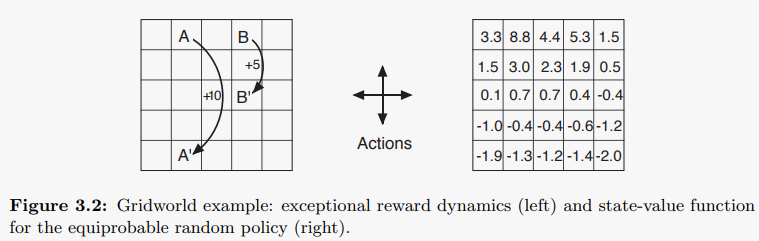
\includegraphics[scale=0.45]{images/suttonbook-fig3.2.png}
    \end{figure}

    \subsection{Answer}

    From the textbook, the state-value function for a policy $\pi$ is defined as,
    \begin{align*}
        v_{\pi}(s) &\doteq \mathbb{E}_{\pi} \left[ G_t \mid S_t = s \right]\\
                   &= \sum_{a} \pi(a \mid s) \sum_{s', r} p(s', r \mid s, a) \left[ r + \gamma v_{\pi}(s') \right]
    \end{align*}

    From Example 3.5, we also know the following given information:
    \begin{itemize}
        \item The action set $A =\{\text{up}, \text{down}, \text{left}, \text{right}\}$ in each state.
        \item An equiprobable random policy is used. Therefore, $\pi(a \mid s) = 0.25$ for all $a \in A$ and $s \in S$.
        \item The reward is always $0$ for all transitions. 
        \item $\gamma = 0.9$.
        \item Any action taken deterministically leads to the expected state, so $p = 1$.
    \end{itemize}
        
    Hence, the state-value function for the center state is,
    \vspace{-0.25cm}\\
    \begin{align*}
        v_{\pi}(s_{\text{center}}) &= \sum_{a} \pi(a \mid s) \sum_{s', r} p(s', r \mid s, a) \left[ r + \gamma v_{\pi}(s') \right]\\
                   &= \pi(\text{up} \mid s) p(s_{\text{up}}, r \mid s, \text{up}) \left[ r + \gamma v_{\pi}(s_{\text{up}}) \right] + 
                   \pi(\text{down} \mid s) p(s_{\text{down}}, r \mid s, \text{down}) \left[ r + \gamma v_{\pi}(s_{\text{down}}) \right]\\
                    & \;\;\; + \pi(\text{left} \mid s) p(s_{\text{left}}, r \mid s, \text{left}) \left[ r + \gamma v_{\pi}(s_{\text{left}}) \right]
                    + \pi(\text{right} \mid s) p(s_{\text{right}}, r \mid s, \text{right}) \left[ r + \gamma v_{\pi}(s_{\text{right}}) \right]\\
                    &= 0.25 \cdot 1 \cdot \left[ 0 + 0.9 \cdot 2.3 \right] + 0.25 \cdot 1 \cdot \left[ 0 + 0.9 \cdot 0.4 \right] + 0.25 \cdot 1 \cdot \left[ 0 + 0.9 \cdot (-0.4) \right] + 0.25 \cdot 1 \cdot \left[ 0 + 0.9 \cdot 0.7 \right]\\
                    &= 0.25 \cdot 0.9 \cdot \left[ 2.3 + 0.4 - 0.4 + 0.7 \right]\\
                    &= 0.25 \cdot 0.9 \cdot 3.0\\
                    &= 0.675 \approx 0.7 \text{ (rounded to one decimal place, as mentioned in prompt)}
    \end{align*}

    Therefore, we see that the Bellman equation holds for the center state, valued at $+0.7$.

\end{homeworkProblem}

\pagebreak

\nobreak\extramarks{Problem 7}{}\nobreak{}

\begin{homeworkProblem}[Problem 7]

    \textbf{(Exercise 3.17)}
    What is the Bellman equation for action values, that
    is, for $q_{\pi}$? It must give the action value $q_{\pi}(s, a)$ in terms of the action
    values, $q_{\pi}(s', a')$, of possible successors to the state-action pair $(s, a)$.\\
    Hint: the backup diagram below corresponds to this equation.
    Show the sequence of equations analogous to (3.14), but for action
    values.

    \begin{figure}[h!]
        \centering
        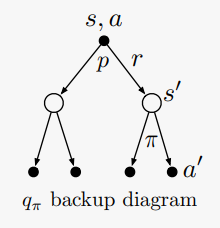
\includegraphics[scale=0.45]{images/suttonbook-qpi-backup-diag.png}
    \end{figure}

    \subsection{Answer}

    From the textbook, the action-value function for a policy $\pi$ is defined as,

    \begin{align*}
        q_{\pi}(s, a) &\doteq \mathbb{E}_{\pi} \left[ G_t \mid S_t = s, A_t = a \right]\\
                   &= \mathbb{E}_{\pi} \left[ \sum_{k=0}^{\infty} \gamma^k R_{t+k+1} \mid S_t = s, A_t = a \right]\\
                   &= \mathbb{E}_{\pi} \left[ R_{t+1} + \gamma \sum_{k=0}^{\infty} \gamma^k R_{t+k+2} \mid S_t = s, A_t = a \right]\\
                   &= \mathbb{E}_{\pi} \left[ R_{t+1} + \gamma G_{t+1} \mid S_t = s, A_t = a \right]\\
                     &= \mathbb{E}_{\pi} \left[ R_{t+1} \mid S_t = s, A_t = a \right] + \gamma \mathbb{E}_{\pi} \left[ G_{t+1} \mid S_t = s, A_t = a \right]\\
    \end{align*}

    Now, let us consider the first and second terms of the above equation separately.\\

    \textbf{First Term}\\
    \vspace{-0.25cm}
    \begin{align*}
        \mathbb{E}_{\pi} \left[ R_{t+1} \mid S_t = s, A_t = a \right] &= \sum_{r \in \mathcal{R}} r \cdot p(r \mid s, a)
        = \sum_{r \in \mathcal{R}} \sum_{s' \in \mathcal{S}} r \cdot p(s', r \mid s, a)
    \end{align*}

    \textbf{Second Term}\\
    \vspace{-0.25cm}
    \begin{align*}
        \gamma \mathbb{E}_{\pi} \left[ G_{t+1} \mid S_t = s, A_t = a \right] &= \gamma \sum_{g \in \mathcal{G}} g \cdot p(g \mid s, a)\\
        &= \gamma \sum_{g \in \mathcal{G}} \sum_{r \in \mathcal{R}} \sum_{s' \in \mathcal{S}} \sum_{a' \in \mathcal{A}} g \cdot p(g \mid s', a') \cdot p(s', r \mid s, a) \cdot \pi(a' \mid s')\\
    \end{align*}
    Where, $\sum_{g \in \mathcal{G}} g \cdot p(g \mid s', a') = \mathbb{E}_{\pi} \left[ G_{t+1} \mid S_{t+1} = s', A_{t+1} = a' \right] = q_{\pi}(s', a')$\\

    Therefore the second term is,

    \begin{align*}
        \gamma \mathbb{E}_{\pi} \left[ G_{t+1} \mid S_t = s, A_t = a \right] &= \gamma\sum_{r \in \mathcal{R}} \sum_{s' \in \mathcal{S}} \sum_{a' \in \mathcal{A}} q_{\pi}(s', a') \cdot p(s', r \mid s, a) \cdot \pi(a' \mid s')\\
    \end{align*}

    Now, combining the first and second terms, we get,

    \begin{align*}
        q_{\pi}(s, a) &=  \sum_{r \in \mathcal{R}} \sum_{s' \in \mathcal{S}} r \cdot p(s', r \mid s, a) + \gamma\sum_{r \in \mathcal{R}} \sum_{s' \in \mathcal{S}} \sum_{a' \in \mathcal{A}} q_{\pi}(s', a') \cdot p(s', r \mid s, a) \cdot \pi(a' \mid s')\\
        q_{\pi}(s, a) &= \sum_{s',r} p(s', r \mid s, a) \left[ r + \gamma\sum_{a'} \pi(a' \mid s') q_{\pi}(s', a') \right]\\
    \end{align*}

    Which is the Bellman equation for action values, i.e., for $q_{\pi}$.

    \subsubsection{Backup Diagram Confirmation}

    This equation can be verified by looking at the backup diagram given in the prompt. The backup diagram
    shows that we start with the state-action pair $(s, a)$. To get to the next state, we are subjected
    to the environment $p(s', r \mid s, a)$. The reward $r$ is added to the discounted return $G_{t+1}$.
    This brings us to our new state, $s'$. At this point, the equation would look as follows,

    \begin{align*}
        q_{\pi}(s, a) &= \sum_{s',r} p(s', r \mid s, a) \left[ r + \gamma v_{\pi}(s') \right]\\
    \end{align*}

    However we still need to eliminate the $v_{\pi}(s')$ term. To do this, we go through our
    policy, $\pi$, to get the action $a'$ that we would take in the state $s'$. Now the equation
    becomes,

    \begin{align*}
        q_{\pi}(s, a) &= \sum_{s',r} p(s', r \mid s, a) \left[ r + \gamma\sum_{a'} \pi(a'\mid s') q_{\pi}(s', a') \right]\\
    \end{align*}

    So, the Bellman equation for action values, i.e., for $q_{\pi}$, is confirmed by the backup diagram.

\end{homeworkProblem}

\pagebreak

\nobreak\extramarks{Problem 8}{}\nobreak{}

\begin{homeworkProblem}[Problem 8]

    \textbf{(Exercise 3.22)}
    Write prompt

    \subsection{Answer}

    TODO

\end{homeworkProblem}

\end{document}